\documentclass[10pt, titlepage, oneside, a4paper]{article}
\usepackage[T1]{fontenc}
\usepackage[titletoc]{appendix}
\usepackage[utf8]{inputenc}
\usepackage{amssymb, graphicx, fancyhdr}
\usepackage{amsmath}
\usepackage{amsthm,algorithm,algorithmic,yhmath,enumitem,lscape}
\usepackage{float}
\usepackage{hyperref, url}
\usepackage{minted}

\newmintinline{c}{}

\addtolength{\textheight}{20mm}
\addtolength{\voffset}{-5mm}
%\renewcommand{\sectionmark}[1]{\markleft{#1}}

\def\inst{Computing Science}
\def\typeofdoc{Assignment 3}
\def\course{5DV149 Datastrukturer och algoritmer}
\def\pretitle{Pretitle}
\def\title{Assignment 3 --- Comparison of Table implementations}
\def\name{Name}
\def\username{CS username}
\def\email{\musername{}@cs.umu.se}
\def\graders{Graders}

\def\mfullpath{\raisebox{1pt}{$\scriptstyle \sim$}\musername/\path}
\def\nfullpath{\raisebox{1pt}{$\scriptstyle \sim$}\nusername/\path}

\newcommand{\R}{\mathbb{R}}
\newcommand{\N}{\mathbb{N}}
\newcommand{\Rn}{\mathbb{R}^n}
\newcommand{\Rnn}{\mathbb{R}^{n \times n}}
\newcommand{\bes}{\begin{equation*}}
\newcommand{\ees}{\end{equation*}}
\newcommand{\be}{\begin{equation}}
\newcommand{\ee}{\end{equation}}
\newcommand{\bms}{\begin{multline*}}
\newcommand{\emults}{\end{multline*}}
\newcommand{\bbm}{\begin{bmatrix}}
\newcommand{\ebm}{\end{bmatrix}}
\newcommand{\eps}{\epsilon}
\newcommand{\fl}{\text{fl}}
\newcommand{\Lp}{{L^p}}
\newcommand{\Ker}{\text{Ker}\,}
\newcommand{\loc}{{\text{loc}}}
\newcommand{\ccinf}{C_c^\infty}
\newcommand{\supp}{\text{supp}}
\newcommand{\dist}{\text{dist}}

\begin{document}
	\begin{titlepage}
		\thispagestyle{empty}
		\begin{large}
			\begin{tabular}{@{}p{\textwidth}@{}}
				\textbf{UMEÅ UNIVERSITET \hfill \today} \\
				\textbf{Department of \inst} \\
				\textbf{\typeofdoc} \\
			\end{tabular}
		\end{large}
		\vspace{25mm}
		\begin{center}
			\LARGE{\pretitle} \\
			\huge{\textbf{\course}}\\
			\vspace{10mm}
			\LARGE{\title} \\
			\vspace{15mm}
            \LARGE{version 1.0} \\
            \vspace{10mm}
			\begin{large}
				\begin{tabular}{ll}
					\textbf{Name} & \name \\
					\textbf{Username} & \username \\
				\end{tabular}
			\end{large}
			\vfill
            \vfill
			\large{\textbf{Graders}}\\
			\mbox{\large{\graders}}
		\end{center}
	\end{titlepage}
    
    % fixar sidfot
	\lfoot{\footnotesize{\name, \username}}
	\rfoot{\footnotesize{\today}}
	\lhead{\sc\footnotesize\title}
	\rhead{\nouppercase{\sc\footnotesize\leftmark}}
	\pagestyle{fancy}
	\renewcommand{\headrulewidth}{0.2pt}
	\renewcommand{\footrulewidth}{0.2pt}

	% skapar innehållsförteckning.
	% Tänk på att köra latex 2ggr för att uppdatera allt
	\pagenumbering{roman}
	\tableofcontents
	% och lägger in en sidbrytning
	\newpage

	\pagenumbering{arabic}

	% i Sverige har vi normalt inget indrag vid nytt stycke
	\setlength{\parindent}{0pt}
	% men däremot lite mellanrum
	\setlength{\parskip}{10pt}

\addtocounter{section}{-1}
\section{Changes}
If this is a resubmission, include a list of changes with respect to
the previous submission.
\section{Introduction}
\label{sec:intro}
% Also possible to use \input{intro.tex} to break down the report into one file per section

\emph{Describe the problem to the reader.} Assume that the reader does not
know the assignment, what do they need to know? (E.g. data structure
interfaces, algorithms, etc.). This section could be split into e.g.
Intro + Theory, Intro + Background etc.\}

\section{Datatypes}
\label{sec:datatypes}
\emph{What methods did you use?} Describe the implementation details for
your implementations of the datatype. Especially discuss how you
handled duplicates. You may organize this section as below.

\subsection{The Table user interface}
\label{sec:orgaade8d0}

Present each of the functions in the user interface.

\subsection{Implementation details}
\label{sec:org9d7104b}

\subsubsection{Table}
\label{sec:org315d8fa}

\emph{Description\ldots{}} \emph{The implementation uses (other data type)\ldots{}} \emph{Duplicates are handled\ldots{}}

\subsubsection{MTFTable}
\label{sec:orgc3e1dd9}

\subsubsection{ArrayTable}
\label{sec:org7b4e5fb}

\subsection{Complexity analysis}
\label{sec:complexity}
Provide a simplifed asymptotic complexity analysis for \emph{one} call to
each function in the user interface for each implementation of the
datatype. The reported information will typically be \(O(1)\), \(O(n)\) or
something similar, so a table is a good presentation. See section
\ref{app:tables} for a further discussion on tables.

Use the table to summarize the complexity. Furthermore, discuss in the
text things that you want to highlight, e.g. why some values are equal
and some or not.

\begin{table}[tbp]
\caption{\label{tab:asympt-complexity}A good caption, e.g., asymptotic complexity for the table operations for the different table implementations.}
\centering
\begin{tabular}{l|l|l|l|l}
 & \texttt{table} & \texttt{mtftable} & \texttt{arraytable} & \ldots{}\\
\hline
\texttt{empty} & \(O(1)\) &  &  & \\
\texttt{isempty} &  &  &  & \\
\texttt{insert} & \(O(n)\) &  &  & \\
\texttt{lookup} &  &  &  & \\
\texttt{remove} &  &  &  & \\
\hline
\texttt{choose\_key} &  &  &  & \\
\texttt{kill} &  &  &  & \\
\texttt{print} &  &  &  & \\
\end{tabular}
\end{table}

\section{Experiments}
\label{sec:experiments}
\emph{What did you do?} How did you set up your experiment? (E.g.  explain
how you ran all \(k\) implementations on the same \(m\) problem sizes.)
How many times did you repeat? What hardware did you run on?  Under
what operating system? If you used an external code package for the
computations, e.g. Matlab, specify its name and version number.
Anything interesting that could affect the results should be
mentioned.

\subsection{User instructions}
\label{sec:userguide}
Explain how the reader can replicate your experiments. As a start,
describe exactly how to compile the source code\footnote{on the linux
system}, e.g.

\begin{verbatim}
gcc -o tabletest -I<path/to/include> <path/to>/table.c tabletest-1.9c
\end{verbatim}

\subsection{Test runs}
\label{sec:testruns}
If you did any test runs, they should be documented, e.g. by screen
dumps. If they are tedious and not important for the general reader,
this section may be deferred to the appendix.

\subsection{The actual experiments}
\label{sec:experiments_detail}
What commands did you use? What experiments were performed? What was
computed? Explain such that the reader can understand the experiments
without looking in the source code. ''The time was computed for
inserting \(n\) elements, for \(n\)=x, y, \ldots{}, z.''

\section{Results}
\label{sec:results}
\emph{What did you find?} For this assignment, refer to slides 45-49 of
lecture note package F06 (Complexity analysis). In particular, \textbf{each
plot should be of the type at the bottom of page 48}. In the caption
and labels, include units, number of runs, how the data was computed
(e.g., mean or median of \(x\) runs), etc. In a real-world report, raw
data would be presented in an appendix.

In particular, generate the following plots:
\begin{enumerate}
\item Two version of a plot for the \texttt{insert} operation. The first version
should include timings for \textbf{all} implemented tables using the most
common \(g(n)\). Thus, some lines may behave different than the
others.  The second version of the plot should only include the
implementations that have the typical \(g(n)\). Be sure to anchor the
bottom y scale to zero.  Figure \ref{fig:fig1} is a poorly
annotated version of such a plot.
\item One plot for the \texttt{remove} operation, similar to the one in Figure
\ref{fig:fig2}. Be sure to anchor the bottom y scale to zero.
\item One plot with the three \texttt{lookup} versions; non-existing, existing, 
skewed similar to Figure \ref{fig:fig3}.
\end{enumerate}

Help the reader to focus by pointing out interesting observations.
However, the results section should be strictly objective, i.e., no
evalution of what is, e.g., ''better''. That is to be left for the
discussion. It is ok to say that ''on data of type x, method b is
fastest'', but not ''method b is better than the others''.


\begin{figure}
\begin{center}
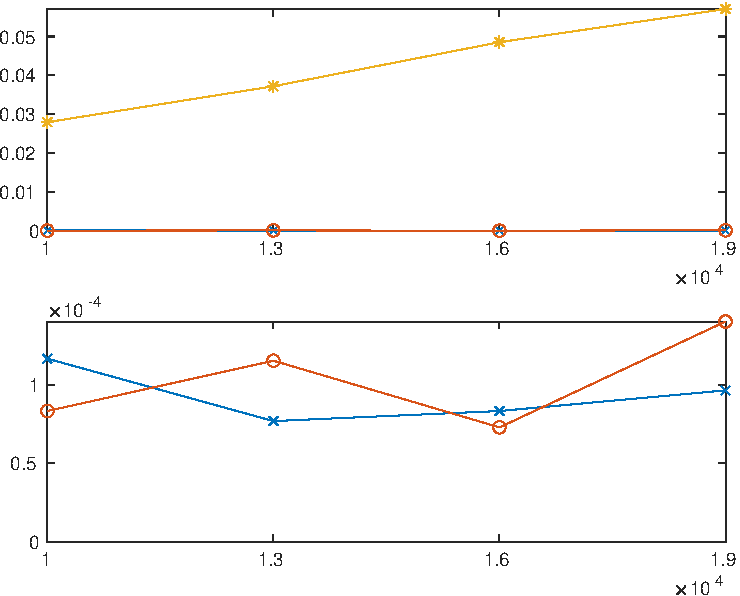
\includegraphics[width=0.75\hsize]{fig1.pdf}
\end{center}
\caption{One}
\label{fig:fig1}
\end{figure}

\begin{figure}
\begin{center}
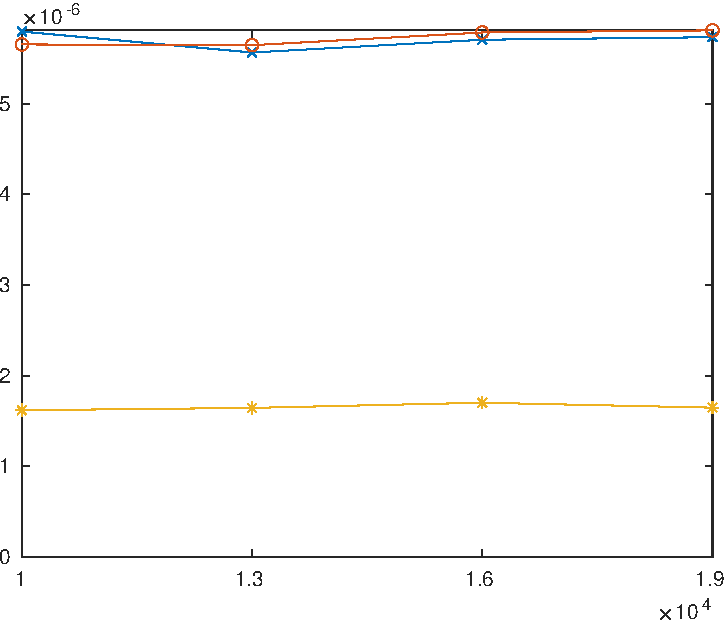
\includegraphics[width=0.75\hsize]{fig2.pdf}
\end{center}
\caption{Two}
\label{fig:fig2}
\end{figure}

\begin{figure}
\begin{center}
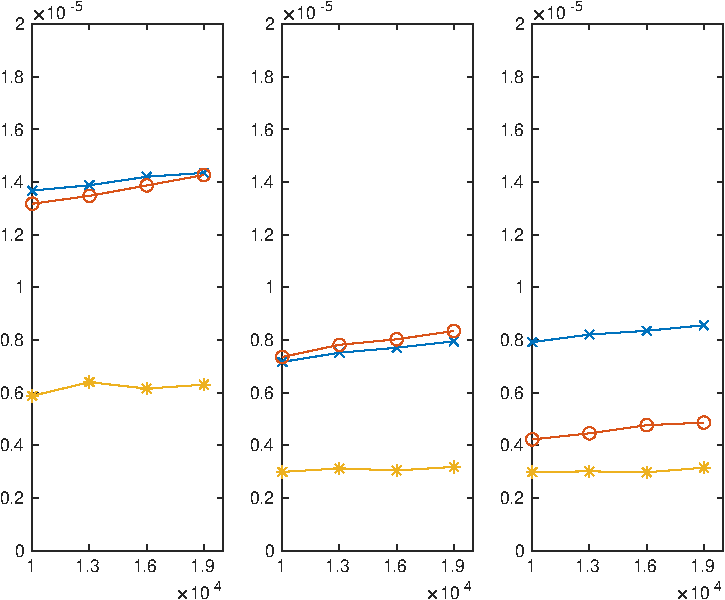
\includegraphics[width=0.75\hsize]{fig3.pdf}
\end{center}
\caption{Three}
\label{fig:fig3}
\end{figure}

\section{Discussion}
\label{sec:discussion}
\subsection{Discussion}
\label{sec:orgb165220}
\emph{What does it mean?} Discuss whether or not the results make sense.
Discuss your methods and their implication on the results (e.g. are
any of the tests misleading?). What limitations does your experiment
have? Are the results in agreement with expectations, or are any
results surprising? Suggest recommendations for future use.

In particular, compare the two list-based implementations. Are the
results similar where the theory suggests they should?  Are the
results different where the theory suggests they should?

Do another comparison between the list-based and array-based
implementations.

Do a third comparison between the unsorted and sorted implementations
(if working in pairs).

\subsection{Conclusion}
\label{sec:orgb4cc8ea}

If your results and recommendations can be briefly summarized, write a
short Conclusion section that expresses your key findings.

\subsection{Future work (optional)}
\label{sec:org793101a}

Did you think of anything interesting to try that you did not have
time to include? If yes, this is the place to 

\subsection{Reflections}
\label{sec:orgbcb9428}

Any personal reflections you did during your work with this
assignment. Anything that was particularly fun, challenging, poorly
specified, surprising, etc.

\clearpage\appendix

\section{Useful \LaTeX{} examples}
\label{app:useful-latex-examples}
Stuff that may be important to some readers, but not all, may be
deferred to an appendix. The same is true for lengthy material that
would disrupt the flow of the document if placed immediately where it
is first referenced. Examples include code listings, file formats,
standards, complete tables of all experiments, etc.

\subsection{Figures}
\label{app:figures}
Figure \ref{fig:image} shows an example of a figure. Exactly \emph{where} (at top
or bottom of a page, on a separate page, or ''here'' in the text) to
put figures/tables is a matter of style. The author of this document
is of the opinion that ''here'' should be avoided at all cost. It
might seem advantageous to have the figure close to the text that
describes it. However, the figure/table should be as self-contained as
possible. In general, it should be possible to read and understand the
body text \emph{without} having to look at the figure. Thus, if you are
forced to write the body text and present the figure such that they
will work independently, your report and writing style will benefit.

As the placement of figures and other floats in \LaTeX{} may shift due to
changes in text, you are encouraged to leave the fine-tuning of image
placement \textbf{until your document is complete}.

\begin{figure}[tbp]
\centering
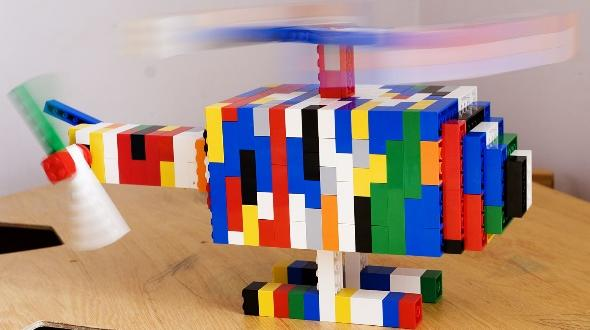
\includegraphics[width=0.7\hsize]{./img.jpg}
\caption{\label{fig:image}A figure/image caption should provide sufficient information to make the figure/image as self-explanatory as possible. The caption should be placed under the figure.}
\end{figure}

If you want to annotate figures from Matlab in \LaTeX{}, or generally
generate figures to impress your mates, the Matlab package \href{https://se.mathworks.com/matlabcentral/fileexchange/22022-matlab2tikz-matlab2tikz?s\_tid=srchtitle}{matlab2tikz}
could be used in conjunction with the \LaTeX{} package PGF/TikZ (\href{https://en.wikibooks.org/wiki/LaTeX/PGF/TikZ}{page on
ikibooks}, \href{https://ctan.org/pkg/pgf}{manual}).

\subsection{Tables}
\label{app:tables}
Tables are often used to present tabulated (no sh*t, sherlock?) data
about the experiment setup, test data, etc., or with results of the
experiments. In the former case, the body text would typically
describe what is common with the data sets and then refer to a table
with detailed information. In the latter case, do not discuss the
structure of the table in the body text! That would just confuse the
reader. Such information belongs to the caption. In general, do not
refer to the table such that the reader cannot continue without
inspecting the table. Instead, summarize enough of the content of the
table to allow the reader to continue to the next paragraph. Also see
Section \ref{sec:results} about how to refer to results.

Data that can better be summarized in the body text should so appear,
e.g., ''The execution time for experiment x was below 2ms. The other
execution times are given in Table x.''

In all cases, consider the number of significant digits! Do not put a
gazillion decimals in your tables just because your code spits it out!
Make the table as easy to read as possible. An example of a stub of a
results table is given in Table \ref{tab:time-table}.

\begin{table}[tbp]
\caption{\label{tab:time-table}A table caption should provide information that helps the reader to understand what data is in the table. Some additional information, e.g., units can also be part of the caption. A table caption should be placed above the table proper. Use as few borders in the table as possible! For instance, adding left and right borders to the table below would make it harder to read.}
\centering
\begin{tabular}{l|l}
\textbf{Table type} & Lookup speed (ms)\\
\hline
MTFTable & x\\
Arraytable & y\\
DListTable & z\\
\end{tabular}
\end{table}

\subsection{Source code}
\label{app:source-code}
If you wish to include any source code in this report, you may use the
\emph{minted} or \emph{listings} packages. The example below shows \emph{minted}.

\begin{minted}[linenos=true=autogobble]{c}
/* Example main */
int main(void) {
    return 0;
}
\end{minted}
\end{document}
